\setchapterpreamble[u]{\margintoc}
\chapter{Second chapter}

\section{One section}
\blindtext

\section{Another section}
\blindtext

In the future I plan to add more options to set the paragraph formatting
(justified or ragged) and the position of the margins (inner or outer in
twoside mode, left or right in oneside mode).\sidenote{As of now,
paragraphs are justified, formatted with \Command{singlespacing} (from
the \Package{setspace} package) and \Command{frenchspacing}.}

I take this opportunity to renew the call for help: everyone is
encouraged to add features or reimplement existing ones, and to send me
the results. You can find the GitHub repository at
\url{https://github.com/fmarotta/kaobook}.

\begin{kaobox}[title=To Do]
  Implement the \Option{justified} and \Option{margin} options. To be
  consistent with the \KOMAScript\xspace style, they should accept a
  simple switch as a parameter, where the simple switch should be
  \Option{true} or \Option{false}, or one of the other standard values for
  simple switches supported by \KOMAScript. See the \KOMAScript\xspace
  documentation for further information.
\end{kaobox}

\blindtext

\begin{table}[ht]
\caption[A useless table]{A useless table.}
\labtab{useless}
\begin{tabular}{ c c c c }
	\toprule
	col1 & col2 & col3 & col 4 \\
	\midrule
	\multirow{3}{4em}{Multiple row} & cell2 & cell3 & cell4\\ &
	cell5 & cell6 & cell7 \\ &
	cell8 & cell9 & cell10 \\
	\multirow{3}{4em}{Multiple row} & cell2 & cell3 & cell4 \\ &
	cell5 & cell6 & cell7 \\ &
	cell8 & cell9 & cell10 \\
	\bottomrule
\end{tabular}
\end{table}


Offset ca be either a measure or a multiple of \Command{baselineskip},
much like with \Command{sidenote}, \Command{marginnote} and
\Command{margintoc}.\todo{Improve this part.} If you are wondering how I
inserted this orange bubble, have a look at the \Package{todo} package.


\section{Wide Figures and Tables}


With the environments \Environment{figure*} and \Environment{table*} you
can insert figures which span the whole page width. For example, here
are a wide figure and a wide table.


\begin{figure*}[h!]
	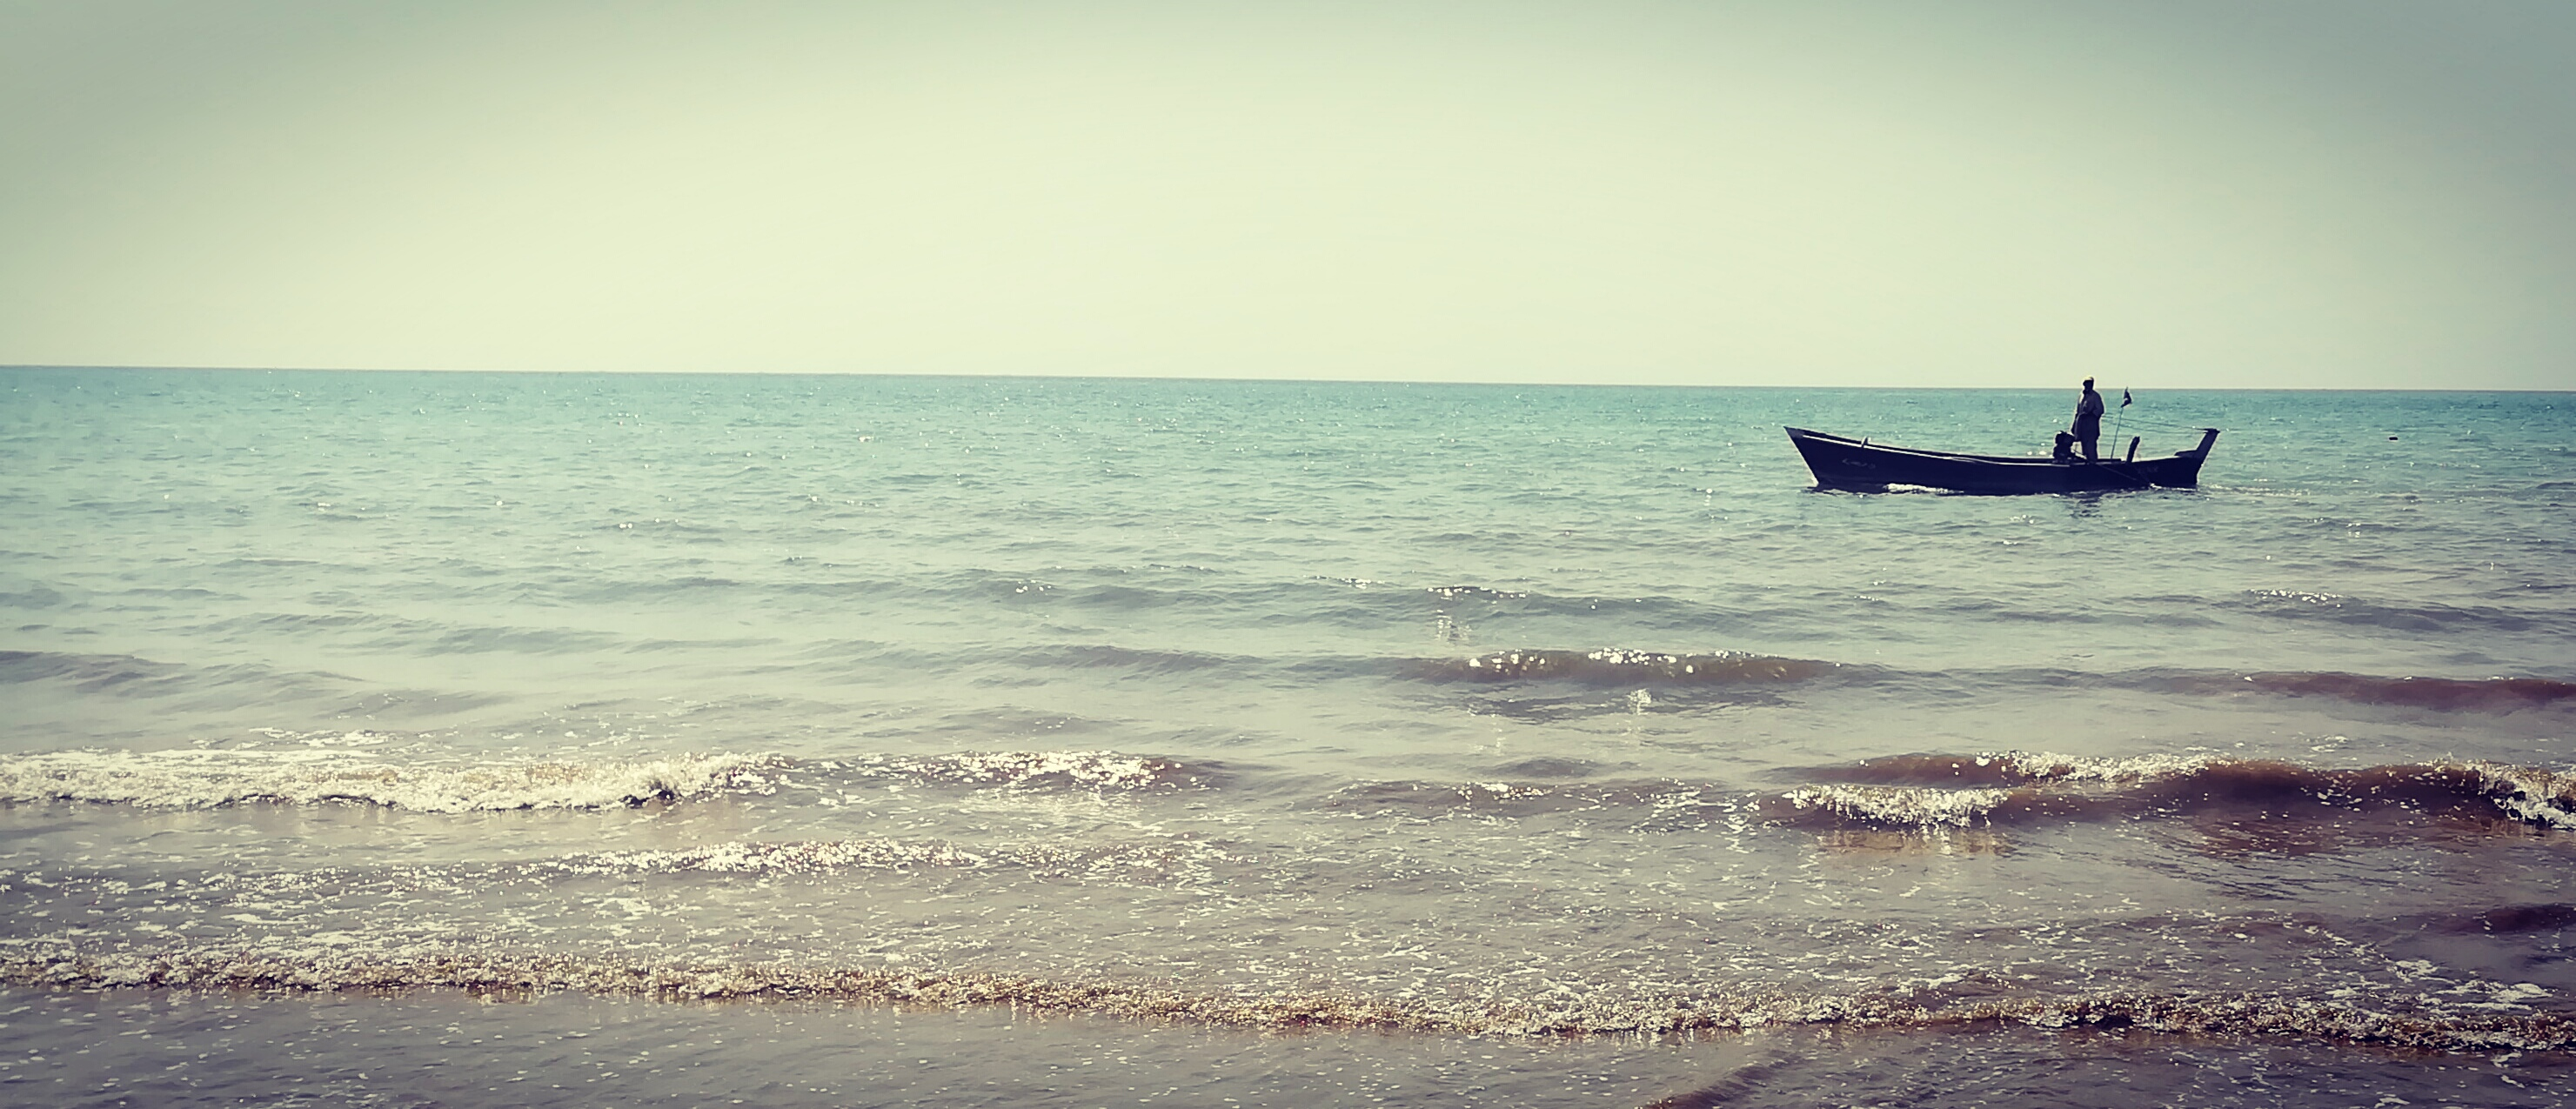
\includegraphics{seaside.jpg}
	\caption[A wide seaside]{A wide seaside, and a wide caption.
		Credits: By Bushra Feroz, CC BY-SA 4.0, \url{https://commons.wikimedia.org/w/index.php?curid=68724647}}
\end{figure*}


\begin{table*}[h!]
    \caption{A wide table with invented data about three people living in the UK. Note that wide figures and tables are centered and their caption also extends into the margin.}
    \begin{tabular}{p{2.0cm} p{2.0cm} p{2.0cm} p{2.0cm} p{2.0cm} p{2.0cm} p{1.5cm}}
        \toprule
        Name    & Surname   & Job       & Salary           & Age   & Height    & Country \\
        \midrule
        Alice   & Red       & Writer    & 4.000 \pounds    & 34    & 167 cm     & England \\
        Bob     & White     & Bartender & 2.000 \pounds    & 24    & 180 cm     & Scotland \\
        Drake   & Green     & Scientist & 4.000 \pounds    & 26    & 175 cm     & Wales \\
        \bottomrule
    \end{tabular}
\end{table*}

\blindtext

\marginnote{
    Here is a random equation, just because we can:
    \begin{equation*}
      x = a_0 + \cfrac{1}{a_1 + \cfrac{1}{a_2 + \cfrac{1}{a_3 + \cfrac{1}{a_4} } } }
    \end{equation*}
}
